\message{ !name(appendices.tex)}
\message{ !name(appendices.tex) !offset(-2) }
\appendix
\section{Appendix: Known unknowns and the reject option}
\label{app:reject}

Formally, let $\mbox{cost}(y^k | y^j)$ encode the penalty for predicting $f(x) = y^k$ when in fact the true label for $x$ is $y^j$. In this case, based on the posterior probability estimates generated by $f(x)$, a model should ideally choose the $y^k$ that minimizes the expected misclassification cost: $$L(x, y^k) = \sum_{y' \in Y} p(y = y' | x) \mbox{cost}(y^k | y')$$

Imagine for simplicity, the setting with balanced misclassification costs, that is, w.l.o.g., $\mbox{cost}(y^k | y^j) = 1$ whenever $y^k \neq y^j$ with $0$ costs for correct label attribution.  In this case, it is straightforward to show~\cite{chow:57,chow:70} that the optimal ``reject'' policy, $\mathcal{A}$ offering a minimum reject rate for a given expected error probability (or, equivalently, minimizing the expected error probability for a given reject rate) is given by:

\begin{equation}
\mathcal{A} = \left\{ x \| \min_c \hat{p}(y = c | x) > q(x) \right\}
\label{eq:rej}
\end{equation}

\begin{figure}[hbt]
\begin{center}
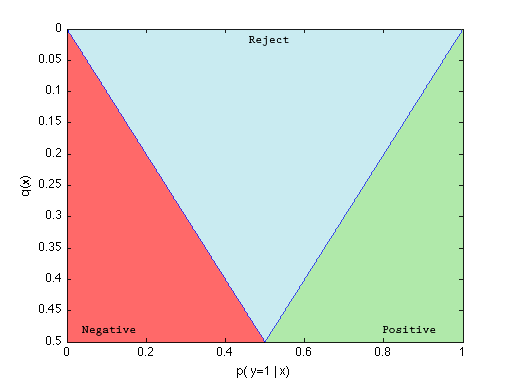
\includegraphics[width= .95 \columnwidth]{plots/reject_decision_bounds_fill.png}
\end{center}
\caption{The reject and classification regions defined by Chow's original classification with a reject option criterion defined in Equation~\ref{eq:rej}}
\label{fig:rejectdecision}
\end{figure}

As would be expected, larger query costs tend to prevent much of the efficacy of the reject option; indeed the reject option would never be exercised with $q(x)>\frac{1}{2}$. (It is optimal to always query the oracle when $q(x) = 0$, thereby yielding zero misclassification risk, assuming a perfect oracle.) Figure~\ref{fig:rejectdecision} presents the decision regions for varying query costs as a function of the posterior probability, $p(y=1|x)$. It is never advantageous to query an oracle once the costs exceed $0.5$.  Of course the uniform misclassification costs assumed by above are seldom realistic. Extending the reject rule of Chow to the case of asymmetric misclassification costs, Herbei and Wegkamp~\cite{herbei:2005} show that the optimal $\mathcal{A}$ is given by: 
\vspace{-0.03in}
\begin{equation}
\mathcal{A} = \left\{ x \| \min_{\hat{y}} L(x, \hat{y}) > q(x) \right\}
\label{eq:costrej}
\end{equation}

\begin{figure}[hbt!]
\begin{center}
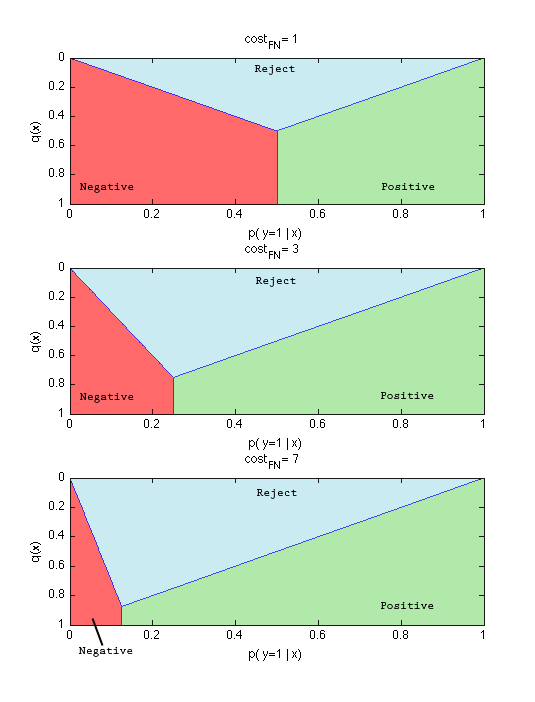
\includegraphics[width= .95 \columnwidth]{plots/cost_reject_decision_bounds_fill.png}
\end{center}
\caption{The reject and classification regions defined by Herbei and Wegkamp's misclassification cost-sensitive classification with a reject option criterion defined in Equation~\ref{eq:costrej} for different false negative costs ($\mbox{cost}_{\mbox{FN}} = \mbox{cost}(0|1)$). }
\label{fig:costdecision}
\end{figure}

As in the case of symmetric cost classification with a reject option, there are certain regions of the posterior/cost space where predictions should be rejected, and where certain labels should be chosen. Figure~\ref{fig:costdecision} presents these regions for a binary classification as a function of the posterior, $p(y=1|x)$ and of a (uniform) label cost, $q(x)$ for three different cost settings. In order to reduce the complexity of the problem being considered, we assume zero costs for correct classifications, and a false positive cost of $1$, eg. $\mbox{cost}(1|0)=1$, varying only $\mbox{cost}(0|1)$. This is equivalent to considering only the ratio of false negative to false positive costs, and re-normalizing.

\message{ !name(appendices.tex) !offset(-41) }
